\section{Проведение эксперимента}
Типичная оптическая схема фурье-спектрометра использует интерферометр Майкельсона (рис. \ref{ust}). 
\begin{figure}[h!]
	\centering
	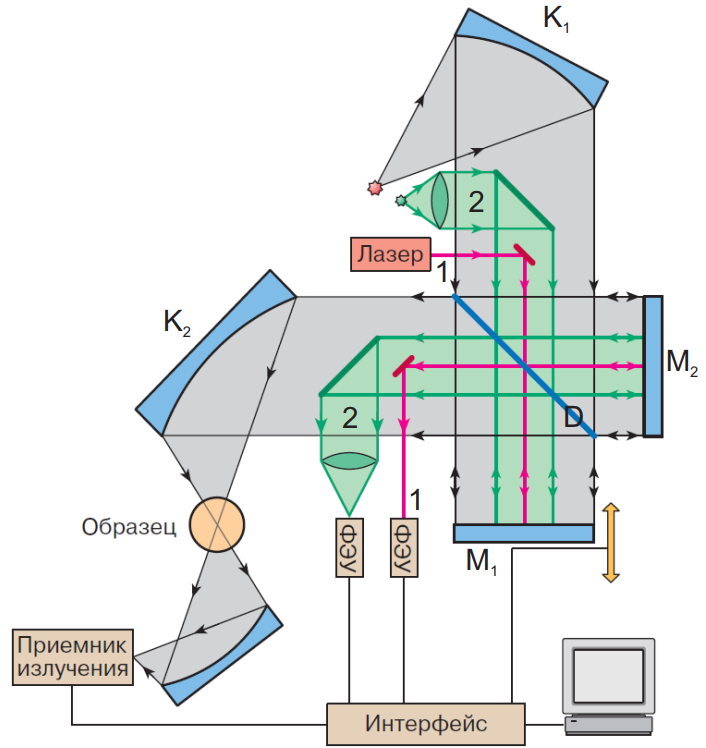
\includegraphics[height=0.7\textheight]{ust}
	\caption{Схема устройства фурье-спектрометра}
	\label{ust}
\end{figure}
Прошедший через входную диафрагму
свет падает на коллиматорное зеркало $K_1$ и параллельным пучком направляется на светоделитель $D$. Светоделитель обычно представляет
собой прозрачную плоскопараллельную пластину с покрытием.
Идеальный светоделитель должен отражать и пропускать ровно по
50\% света и не иметь поглощения во всей спектральной области работы
прибора. Отклонение от этого требования снижает эффективность его
работы. Однако реализовать такое требование очень трудно, особенно
в инфракрасной области спектра, где длина волны может меняться в
десятки раз. Поэтому в фурье-спектрометрах используют сменные светоделители. Область работы каждого светоделителя бывает достаточно
широкой: она обычно допускает пятикратное изменение длины волны,
что гораздо больше, чем для призм или дифракционных решеток. В
области низких частот, когда длина волны превышает 25 мкм (микроволновая область), в качестве светоделителей используют полимерные
пленки.

После светоделителя прошедший и отраженный пучки попадают на
отражающие зеркала $M_1$ и $M_2$, требования к качеству и стабильности
которых в интерферометрах очень высоки: их поверхность не должна
отклоняться от идеальной более чем на 1/20 длины волны, отвечающей коротковолновой границе работы прибора. В последнее время
вместо плоских пластин стали использовать тетраэдрические отражатели, составленные из трех взаимно перпендикулярных пластин. Такая
конструкция позволила снизить требование к стабильности, поскольку для тетраэдрического отражателя падающий и отраженный лучи
остаются параллельными при его наклонах.

Выходящее из интерферометра излучение фокусируется зеркальным объективом $K_2$ в месте, куда помещается образец, если исследуются спектры поглощения. После этого свет фокусируется на приемнике излучения.

Важным элементом оптической схемы является система измерения
разности хода между зеркалами интерферометра. Для этой цели в него вводится излучение одномодового
лазера (обычно это лазер He–Ne), которое в прецизионных приборах
дополнительно стабилизируется. После прохождения через интерферометр монохроматический пучок генерирует при движении зеркала синусоидальный сигнал на специальном приемнике. Период синусоиды
равен длине волны лазерного излучения $\lambda$. Этот сигнал после преобразования используется в создании командных импульсов для считывания показаний с приемника излучения в приемно-усилительной
системе интерферометра при смещении подвижного зеркала на расстояние, равное $\lambda$ или кратное этой величине. Благодаря такой системе фурье-спектрометр становится прибором с высокой точностью
измерений частот спектральных линий, причем точность определяется
точностью определения частоты генерации опорного лазера.

Иногда в схему встраивается еще один интерферометр — интерферометр белого света. Он используется
для определения нулевой разности хода между зеркалами. Дело в том,
что для излучения с широким спектральным составом при нулевой разности хода световые колебания всех частот при сложении пучков на
выходе интерферометра будут иметь одну и ту же фазу в разных пучках
и в этом случае будут складываться амплитуды световых колебаний.
Если разность хода велика, разности фаз колебаний для разных частот
будут практически случайными и тогда складываются энергии волн с
разными частотами, что дает вдвое меньшую освещенность на приемнике излучения, чем в случае сложения синхронизированных волн.
По этой причине при перемещении подвижного зеркала в сигнале с
приемника интерферометра белого света при нулевой разности хода
возникает резкий пик.

